\chapter{Experimental Setup and Results}
\label{chap:experiments}

This chapter replaces the single-hand-verified-query benchmark of
earlier drafts with the project's \texttt{10q} suite: ten held-out,
genre-diverse questions, each run ten times per method for statistical
robustness, from the repository branch
\texttt{agent/consolidate-four-method-benchmarks}
(\texttt{benchmarks/10q/}). This directly addresses the ``threats to
validity'' limitation flagged in earlier analysis of this project --
that conclusions rested on one query -- while keeping every other
experimental control (dataset provenance, evaluation harness, metric
definitions) unchanged from Chapter~\ref{chap:architecture}.

\section{The 10-Question Benchmark Suite}
\label{sec:10q-suite}

\subsection{Dataset construction}
All four suites in the repository (\texttt{1q}, \texttt{3q}, \texttt{5q},
\texttt{10q}) draw controlled, balanced per-question subdatasets from
the same canonical $\sim$25{,}000-row IMDb corpus used throughout this
project (structured movie metadata joined to one free-text review per
movie, restored from the original Stanford IMDb review split and the
IMDb non-commercial title/crew/name datasets). For the \texttt{10q}
suite, each of the ten questions is paired with its own $100$-movie
candidate pool, constructed with a fixed, auditable composition:
\begin{itemize}
  \item $12$ true positives (satisfy both the structured and the
        semantic predicate);
  \item $28$ structured-semantic negatives (satisfy the structured
        predicate, fail the semantic one -- the ``hard'' negatives a
        row-wise semantic filter must reject correctly);
  \item $30$ semantic-only distractors (fail the structured predicate
        but would arguably satisfy the semantic one -- probing whether
        an implementation actually applies structured pushdown, or
        leaks these in through a join that ignores it, as in
        Section~\ref{sec:trummer-baseline});
  \item $30$ double negatives (fail both predicates).
\end{itemize}
Every row's \texttt{structured\_match} and \texttt{semantic\_label} are
recorded in an \texttt{annotations.csv} data dictionary, with an
\texttt{evidence\_excerpt} and \texttt{annotation\_rationale} per row, so
every label is auditable back to a specific review span -- directly
addressing the earlier-flagged hardcoded-gold-count fragility
(Section~\ref{sec:eval-harness}) by construction rather than by
discipline alone.

\subsection{The ten questions}
Table~\ref{tab:10q-questions} lists the ten questions, spanning seven
genres and five difficulty levels (medium to very-hard, assigned by the
question designer based on predicate specificity and expected
vocabulary overlap with review text). Every question has the same
structural shape as the others (100 candidates, 40 structured
candidates, 12 ground truth), which lets us compare methods
\emph{within} a controlled cost budget while still varying the semantic
task substantially.

\begin{table}[h]
\centering\small
\begin{tabular}{clp{7.6cm}}
\toprule
Q & Difficulty & Semantic task \\
\midrule
1 & medium & Animated-film humor (funny/hilarious reviews) \\
2 & medium\_hard & Modern-drama ($\ge$1990) acting/performance praise \\
3 & hard & Feature-length (90--130min) romantic chemistry \\
4 & medium\_hard & Long-action ($\ge$100min) excitement/suspense \\
5 & very\_hard & Mystery ending/twist approval \\
6 & medium\_hard & Music/Musical soundtrack and score praise \\
7 & medium\_hard & Pre-2000 drama emotional impact \\
8 & hard & Science-fiction intellectual depth \\
9 & medium\_hard & Documentary informational value \\
10 & medium & Family ($<$121min) entertainment value \\
\bottomrule
\end{tabular}
\caption{The ten held-out questions of the \texttt{10q} suite. Every
question has 100 candidates, 40 structured candidates, and 12
ground-truth movies (\texttt{manifest.json}).}
\label{tab:10q-questions}
\end{table}

\subsection{Run configuration}
Each of the four methods (SUQL baseline/V1, Trummer baseline/V1) is run
$10$ times per question against Ollama-served models -- a cheap model
(Gemma~4, \texttt{e2b}) for both cascades' Stage~1, and a larger
expensive model (Gemma~4, \texttt{26b}) for all four methods' Stage~2 /
baseline evaluation -- and results are averaged first per question
(\texttt{comparison.csv}) and then across all ten questions
(\texttt{aggregate.csv}), which is the source of every number in this
chapter.

\section{Aggregate Results}
\label{sec:10q-aggregate}

\begin{table}[h]
\centering\small
\begin{tabular}{lrrrr}
\toprule
Metric & SUQL base. & SUQL V1 & Trummer base. & \textbf{Trummer V1} \\
\midrule
Wall time (s) & 115.57 & 923.60 & 71.28 & \textbf{35.05} \\
LLM calls     & 117.08 & 70.05  & 96.87 & \textbf{10.00} \\
\ \ cheap calls     & 0      & 40.00  & 0     & 5.00 \\
\ \ expensive calls & 117.08 & 30.05  & 96.87 & 5.00 \\
\ \ cheap seconds   & 0      & 834.32 & 0     & 21.08 \\
\ \ expensive seconds & 115.57 & 89.25 & 71.28 & 13.98 \\
\bottomrule
\end{tabular}
\caption{Cost per question, averaged over 10 questions $\times$ 10
repetitions (\texttt{aggregate.csv}).}
\label{tab:cost-chapter5}
\end{table}

\begin{table}[h]
\centering\small
\begin{tabular}{lrrrr}
\toprule
Metric & SUQL base. & SUQL V1 & Trummer base. & \textbf{Trummer V1} \\
\midrule
Precision & 0.683 & 0.709 & 0.655 & \textbf{0.810} \\
Recall    & 0.758 & \textbf{0.808} & 0.408 & 0.750 \\
F1        & 0.678 & 0.696 & 0.444 & \textbf{0.757} \\
\bottomrule
\end{tabular}
\caption{Quality per question, averaged over 10 questions $\times$ 10
repetitions (best variant per row in bold).}
\label{tab:quality-chapter5}
\end{table}

\begin{table}[h]
\centering\small
\begin{tabular}{lrrr}
\toprule
Comparison & $\Delta$Precision & $\Delta$Recall & $\Delta$F1 \\
\midrule
SUQL V1 vs.\ SUQL baseline       & $+3.87\%$  & $+6.59\%$  & $+2.65\%$ \\
Trummer V1 vs.\ Trummer baseline & $+23.63\%$ & $+83.67\%$ & $+70.38\%$ \\
Trummer V1 vs.\ SUQL V1          & $+14.21\%$ & $-7.22\%$  & $+8.78\%$ \\
\bottomrule
\end{tabular}
\caption{Relative quality, derived from Table~\ref{tab:quality-chapter5}.}
\label{tab:quality-ratios}
\end{table}

\begin{table}[h]
\centering\small
\begin{tabular}{lrr}
\toprule
Comparison & Wall time & LLM calls \\
\midrule
SUQL V1 vs.\ SUQL baseline       & $7.99\times$ slower & $0.598\times$ (40.2\% fewer) \\
Trummer V1 vs.\ Trummer baseline & $2.03\times$ faster & $0.103\times$ (89.7\% fewer) \\
Trummer V1 vs.\ SUQL V1          & $26.3\times$ faster & $0.143\times$ ($\approx 1/7$) \\
\bottomrule
\end{tabular}
\caption{Relative cost, derived from Table~\ref{tab:cost-chapter5}.}
\label{tab:cost-ratios}
\end{table}

\section{Per-Question Breakdown}
\label{sec:per-question}

Table~\ref{tab:per-question-f1} shows F1 for all four methods on each of
the ten questions individually. Two patterns emerge that the single-query
benchmark of earlier drafts could not reveal.

\begin{table}[h]
\centering\small
\begin{tabular}{clrrrr}
\toprule
Q & Semantic task & SB & SV1 & TB & \textbf{TV1} \\
\midrule
1  & Animation humor              & 0.762 & 0.774 & 0.375 & \textbf{0.783} \\
2  & Modern-drama acting          & 0.649 & 0.649 & 0.645 & 0.615 \\
3  & Romance chemistry            & 0.267 & 0.286 & 0.154 & \textbf{0.917} \\
4  & Long-action excitement       & 0.667 & 0.720 & 0.500 & \textbf{0.870} \\
5  & Mystery ending approval      & 0.692 & 0.714 & 0.667 & \textbf{0.857} \\
6  & Music/Musical soundtrack     & 0.667 & \textbf{0.667} & 0.312 & 0.519 \\
7  & Pre-2000 drama emotion       & 0.667 & 0.700 & 0.375 & \textbf{0.737} \\
8  & Sci-Fi intellectual depth    & \textbf{0.917} & 0.846 & 0.444 & 0.857 \\
9  & Documentary informational    & 0.846 & \textbf{0.957} & 0.444 & 0.917 \\
10 & Family entertainment value   & \textbf{0.647} & \textbf{0.647} & 0.526 & 0.500 \\
\midrule
\multicolumn{2}{l}{mean} & 0.678 & 0.696 & 0.444 & \textbf{0.757} \\
\multicolumn{2}{l}{min}  & 0.267 & 0.286 & 0.154 & \textbf{0.500} \\
\multicolumn{2}{l}{max}  & 0.917 & 0.957 & 0.667 & \textbf{0.917} \\
\multicolumn{2}{l}{std.\ dev.} & 0.171 & 0.174 & 0.153 & 0.159 \\
\bottomrule
\end{tabular}
\caption{Per-question F1 (SB = SUQL baseline, SV1 = SUQL~V1, TB =
Trummer baseline, TV1 = Trummer~V1), from \texttt{comparison.csv}.}
\label{tab:per-question-f1}
\end{table}

\textbf{Trummer~V1's floor, not just its average, is highest.} Every
method's mean F1 is pulled down by at least one hard question (Q3,
Romance chemistry, is the worst question for three of the four methods),
but Trummer~V1's \emph{minimum} across all ten questions ($0.500$, on
Q10) is higher than every other method's minimum -- SUQL baseline and
SUQL~V1 both drop to the $0.27$--$0.29$ range on Q3, and the Trummer
baseline drops to $0.154$ on the same question. Trummer~V1 is the only
method that never catastrophically fails on a held-out question in this
suite, which matters more for a deployed system than the mean alone: a
system that is usually excellent but occasionally very bad is a worse
production dependency than one that is consistently good.

\textbf{Q3 (Romance chemistry) is the clearest illustration of what the
cascade's escalation step buys.} Both non-cascaded baselines are
extremely weak here (SUQL baseline F1 $0.267$, Trummer baseline
$0.154$) -- ``praising the characters' chemistry or relationship'' is
exactly the kind of paraphrase-heavy, vocabulary-mismatched predicate
that a single judgment pass (row-wise or block-joined) struggles with.
SUQL~V1's row-wise escalation barely helps ($0.286$), consistent with
Section~\ref{sec:theory-cost}'s finding that its cheap stage adds
latency without a batching-driven accuracy benefit here, while
Trummer~V1 jumps to $0.917$ -- the batched cheap pass filters out the
bulk of clear negatives cheaply, and the expensive verification step is
reserved for, and evidently effective on, the residual ambiguous cases
this predicate produces in volume.

\section{Benchmark Visualizations}
\label{sec:imdb-plots}

This section reproduces, one at a time, the six summary plots the
benchmark harness generates directly from \texttt{aggregate.csv} and
\texttt{comparison.csv} for the run analyzed in this chapter
(\texttt{heldout\_diverse\_10q\_10rep\_gemma4\_e2b\_26b\_kraken\_20260722}).
Panels (a)--(d) restate numbers already tabulated in
Tables~\ref{tab:cost-chapter5}--\ref{tab:quality-ratios}; panels (e)--(f)
add a \$-cost view (recorded model service time $\times$
\$3.00/accelerator-hour, token usage not recorded) not available from
the tables alone.

\begin{figure}[h]
\centering

\includegraphics[width=0.85\textwidth]{figs/imdb10q/01_quality.png}
\caption{IMDb \texttt{10q}: precision, recall, and F1 by method.}
\label{fig:imdb-quality}
\end{figure}

Figure~\ref{fig:imdb-quality} shows precision/recall/F1 side by side for
all four methods. SUQL~V1 has the tallest recall bar of the four
($0.808$), consistent with its recall-first cheap-stage design; Trummer
baseline is visibly the weakest method on every bar, with recall
collapsing to $0.408$ against a comparable precision ($0.655$) --
exactly the incomplete-coverage failure mode of
Section~\ref{sec:trummer-baseline}. Trummer~V1's three bars are the
most balanced and, on F1 (purple), the tallest of the four.

\begin{figure}[h]
\centering

\includegraphics[width=0.85\textwidth]{figs/imdb10q/02_time.png}
\caption{IMDb \texttt{10q}: mean wall time per question, cheap vs.\
expensive stage.}
\label{fig:imdb-time}
\end{figure}

Figure~\ref{fig:imdb-time} is the clearest single visual in this report
of the mechanism Section~\ref{sec:theory-cost} proves analytically:
SUQL~V1's bar is by far the tallest ($923.6$s total), and it is
\emph{dominated by its own cheap stage} (green, $77\%$ of the bar) --
the cheap probe is not actually cheap in wall-clock terms. Trummer~V1's
bar is the shortest ($35.1$s) and mostly cheap-stage time (green,
$83\%$), but at a small fraction of SUQL~V1's absolute height, because
Trummer~V1's cheap stage is batched.

\begin{figure}[h]
\centering

\includegraphics[width=0.85\textwidth]{figs/imdb10q/03_calls.png}
\caption{IMDb \texttt{10q}: mean LLM calls per question, cheap vs.\
expensive stage.}
\label{fig:imdb-calls}
\end{figure}

Figure~\ref{fig:imdb-calls} shows the same cheap/expensive split for
call counts rather than time. SUQL~V1's total calls ($70.0$) are lower
than SUQL baseline's ($117.1$), unlike the time comparison above -- a
visual reminder that SUQL~V1 trades calls for time, not both at once
(Table~\ref{tab:cost-ratios}). Trummer~V1 needs only $10.0$ calls
total, split evenly between its cheap batched pass ($5.0$) and its
expensive verification pass ($5.0$).

\begin{figure}[h]
\centering

\includegraphics[width=0.85\textwidth]{figs/imdb10q/04_best_solution.png}
\caption{IMDb \texttt{10q}: recall vs.\ wall time, bubble size
indicating overall quality/cost balance; the harness's own
best-solution annotation is Trummer~V1.}
\label{fig:imdb-best}
\end{figure}

Figure~\ref{fig:imdb-best} plots recall against wall time for all four
methods at once. Trummer~V1 (outlined bubble) sits in the
bottom-left -- low time, competitive recall -- while SUQL~V1 sits at
the far right ($923.6$s) despite a similar recall to SUQL baseline,
visually isolating SUQL~V1's wall-time regression from its recall
profile. Trummer baseline sits lowest on the recall axis, consistent
with Figure~\ref{fig:imdb-quality}.

\begin{figure}[h]
\centering

\includegraphics[width=0.85\textwidth]{figs/imdb10q/05_cost_by_approach.png}
\caption{IMDb \texttt{10q}: estimated \$-cost per question
(recorded model service time $\times$ \$3.00/accelerator-hour).}
\label{fig:imdb-cost}
\end{figure}

Figure~\ref{fig:imdb-cost} converts Figure~\ref{fig:imdb-time} into
dollar terms. At \$3.00/accelerator-hour, SUQL~V1 costs \$0.770 per
question -- more than \emph{twenty-six times} Trummer~V1's \$0.029 --
while SUQL baseline (\$0.096) and Trummer baseline (\$0.059) sit in
between. The per-call figures printed under each bar also show the
``cheap'' stage costing \emph{more} per call than the expensive stage
for both cascades: \$0.01738 vs.\ \$0.00248 for SUQL~V1 ($7.0\times$),
and \$0.00351 vs.\ \$0.00233 for Trummer~V1 ($1.5\times$). Because this
harness's \$-cost is simply recorded service time multiplied by a flat
rate, these ratios exactly match the cheap/expensive \emph{time} ratios
already reported in Section~\ref{sec:worked-instantiation}
($7.02\times$ and $1.51\times$), not an independent pricing signal.

\begin{figure}[h]
\centering

\includegraphics[width=0.85\textwidth]{figs/imdb10q/06_cost_vs_f1.png}
\caption{IMDb \texttt{10q}: cost--F1 Pareto frontier.}
\label{fig:imdb-pareto}
\end{figure}

Figure~\ref{fig:imdb-pareto} plots F1 against \$-cost directly.
\textbf{Trummer~V1 is the unique non-dominated point} -- it has both
the lowest cost \emph{and} the highest F1 of all four methods
simultaneously, so it alone strictly dominates the other three (unlike
the Amazon experiments below, where two points share the frontier).
This closes the open question from an earlier revision of this report:
the near-identical SUQL~V1 \$-costs later observed across the Qwen and
Gemma Amazon runs (Section~\ref{sec:amazon-model-comparison-2}) are not
evidence of a shared underlying model -- they simply reflect that
\$-cost here is a deterministic linear function of recorded time, so
any two runs with similar per-call \emph{latency} show similar
\$-costs regardless of which model produced that latency.

\section{Cross-Domain Validation: Amazon Data}
\label{sec:amazon-experiment}

All \texttt{10q} results so far are on IMDb movies. Three follow-up
experiments test whether the cascade's cost advantage, and the
theoretical margin condition of Section~\ref{sec:theory-cost}, hold on
a different domain: (1) a single-question, wide pool-size sweep on
Amazon product reviews under Gemma (\emph{dense}/\emph{calibfrac}),
designed to stress-test the crossover claim directly as $n$ grows; (2)
a full ten-question \emph{Amazon Fashion} suite under the same Gemma
pair, built in the same ten-question-averaged format as the IMDb suite
above, so it can be compared to Table~\ref{tab:quality-chapter5}
directly rather than only to a single pool-size point; and (3) a
five-question Amazon suite under a Qwen cheap/expensive pair, testing
whether the findings are specific to Gemma.

\subsection{IMDb vs.\ Amazon Fashion: Matched Suite, Same Model}
\label{sec:imdb-vs-amazon-fashion}

Table~\ref{tab:imdb-vs-amazon} compares the IMDb \texttt{10q} suite
(Chapter~\ref{chap:experiments}) against a new Amazon Fashion
\texttt{10q} suite -- same model pair, same ten-question-averaged
methodology, differing only in domain. This is a materially better
comparison than the single pool-size point used in an earlier revision
of this report, and it revises one conclusion drawn from that point
estimate: with the full ten-question average, \textbf{Trummer~V1's F1
advantage over SUQL baseline does not replicate on Amazon Fashion} -- it
is a small \emph{loss} ($-4.3\%$), not the modest gain the single
pool-size point had suggested.

\begin{figure}[h]
\centering

\includegraphics[width=0.85\textwidth]{figs/amazon_fashion_gemma/01_quality.png}
\caption{Amazon Fashion \texttt{10q}, Gemma: precision, recall, F1
(error bars: std.\ dev.\ across repetitions).}
\label{fig:amzf-quality}
\end{figure}

Figure~\ref{fig:amzf-quality} shows all four methods within a much
narrower quality band than on IMDb (Figure~\ref{fig:imdb-quality}):
three of four F1 bars sit between $0.776$ and $0.835$. The exception is
Trummer baseline, whose precision collapses to $0.330$ despite the
\emph{highest} recall of any method or domain seen so far ($0.967$) --
the opposite imbalance from its IMDb profile (precision $0.655$,
recall $0.408$), discussed further below.

\begin{figure}[h]
\centering

\includegraphics[width=0.85\textwidth]{figs/amazon_fashion_gemma/02_time.png}
\caption{Amazon Fashion \texttt{10q}, Gemma: mean wall time, cheap vs.\
expensive stage.}
\label{fig:amzf-time}
\end{figure}

Figure~\ref{fig:amzf-time} shows the same qualitative pattern as IMDb
(Figure~\ref{fig:imdb-time}): SUQL~V1's bar is tallest ($48.7$s) and
majority cheap-stage (green, $77\%$), while Trummer~V1's is shortest
($11.8$s). The absolute gap is smaller here (SUQL baseline itself is
only $19.6$s, versus $115.6$s on IMDb), which is why the \emph{relative}
speedup Trummer~V1 achieves over baseline is weaker on this domain
(Table~\ref{tab:imdb-vs-amazon}).

\begin{figure}[h]
\centering

\includegraphics[width=0.85\textwidth]{figs/amazon_fashion_gemma/03_calls.png}
\caption{Amazon Fashion \texttt{10q}, Gemma: mean LLM calls, cheap vs.\
expensive stage.}
\label{fig:amzf-calls}
\end{figure}

Figure~\ref{fig:amzf-calls} is where SUQL~V1's Amazon-Fashion-specific
failure is easiest to see: its bar ($78.3$ calls) is \emph{taller} than
SUQL baseline's ($49.2$), the reverse of the IMDb pattern
(Figure~\ref{fig:imdb-calls}), where SUQL~V1 used \emph{fewer} calls
than its baseline. Trummer~V1 again needs the fewest calls overall
($13.0$).

\begin{figure}[h]
\centering

\includegraphics[width=0.85\textwidth]{figs/amazon_fashion_gemma/04_best_solution.png}
\caption{Amazon Fashion \texttt{10q}, Gemma: recall vs.\ wall time,
harness best-solution annotation is Trummer~V1.}
\label{fig:amzf-best}
\end{figure}

Figure~\ref{fig:amzf-best} places SUQL~V1 at the far right on time
while its recall bubble sits no higher than SUQL baseline's or
Trummer~V1's -- visually, SUQL~V1 buys no recall advantage for its
much larger time cost on this domain, unlike IMDb where it at least
had the single highest recall bubble.

\begin{figure}[h]
\centering

\includegraphics[width=0.85\textwidth]{figs/amazon_fashion_gemma/05_cost_by_approach.png}
\caption{Amazon Fashion \texttt{10q}, Gemma: estimated \$-cost per
question.}
\label{fig:amzf-cost}
\end{figure}

Figure~\ref{fig:amzf-cost} puts SUQL~V1 as the most expensive method in
dollar terms (\$0.0406) despite Trummer baseline having no cheap stage
at all (\$0.0306) -- SUQL~V1's combination of more calls \emph{and} a
pricier cheap stage compounds here. Trummer~V1 remains cheapest
(\$0.0098).

\begin{figure}[h]
\centering

\includegraphics[width=0.85\textwidth]{figs/amazon_fashion_gemma/06_cost_vs_f1.png}
\caption{Amazon Fashion \texttt{10q}, Gemma: cost--F1 Pareto frontier.}
\label{fig:amzf-pareto}
\end{figure}

Figure~\ref{fig:amzf-pareto} shows \emph{two} non-dominated points here
-- Trummer~V1 and SUQL baseline -- rather than the single dominant
point IMDb showed (Figure~\ref{fig:imdb-pareto}): SUQL baseline has
slightly higher F1 ($0.835$ vs.\ $0.799$) at slightly higher cost
($\$0.0164$ vs.\ $\$0.0098$), so neither strictly dominates the other.
SUQL~V1 and Trummer baseline are both strictly dominated.

\begin{table}[h]
\centering\small
\begin{tabular}{lrr}
\toprule
 & IMDb \texttt{10q} & Amazon Fashion \texttt{10q} \\
\midrule
\multicolumn{3}{l}{\emph{Trummer~V1 vs.\ SUQL baseline}} \\
$\Delta$F1     & $+11.7\%$  & $-4.3\%$ \\
$\Delta$calls  & $-91.5\%$  & $-73.6\%$ \\
$\Delta$time   & $-69.7\%$  & $-39.8\%$ \\
\midrule
\multicolumn{3}{l}{\emph{SUQL~V1 vs.\ SUQL baseline}} \\
$\Delta$F1     & $+2.7\%$   & $-7.1\%$ \\
$\Delta$calls  & $-40.2\%$  & $+59.1\%$ \\
$\Delta$time   & $+699\%$   & $+148\%$ \\
\bottomrule
\end{tabular}
\caption{Same model (Gemma), same suite design (10 questions averaged),
different domain.}
\label{tab:imdb-vs-amazon}
\end{table}

Three findings follow. \textbf{First}, absolute quality is
substantially higher on Amazon Fashion (SUQL baseline F1 $0.835$) than
on IMDb ($0.678$) -- consistent with product reviews being a less
ambiguous, less paraphrase-heavy signal than movie reviews for the
predicates tested here, though this is one ten-question suite per
domain, not a controlled difficulty match. \textbf{Second}, cost
dominance transfers directionally but is \emph{weaker}: Trummer~V1
still cuts calls substantially ($-73.6\%$) and time ($-39.8\%$), but by
less than on IMDb, because SUQL baseline itself is already cheap on
Amazon Fashion ($49.2$ calls vs.\ IMDb's $117.1$), leaving less
headroom for the cascade to reclaim. \textbf{Third}, and most
importantly, \emph{SUQL~V1 is strictly dominated by its own baseline on
Amazon Fashion} -- worse on calls ($+59\%$), time ($+148\%$), \emph{and}
F1 ($-7.1\%$) simultaneously -- unlike on IMDb, where it at least traded
time for a small quality gain. This matches, and strengthens with a
properly-matched suite, the same finding from the Qwen run below
(\S\ref{sec:amazon-model-comparison-2}): \textbf{SUQL~V1's viability
appears specific to the IMDb/Gemma combination it was developed
against, not a general property of the cascade design.} Trummer~V1's
structured pushdown plus batching, by contrast, remains the best or
co-best design point in both domains.

\subsection{Scaling and Reliability Validation}
\label{sec:amazon-scaling}

A second, complementary experiment sweeps a single Amazon question
across a much wider pool-size range ($n=100$ to $n=300$, $100$--$150$
repetitions per point) specifically to test the crossover behavior of
Proposition~\ref{prop:crossover} as $n$ grows, rather than to compare
quality across questions. Two calibration regimes were run: a
\emph{dense} run with fixed $K_{\mathrm{calls}}=20$, and an adversarial
\emph{calibfrac} run where calibration is re-paid at a constant $20\%$
of $n$ (so the $K/n$ term never vanishes).

\begin{figure}[h]
\centering
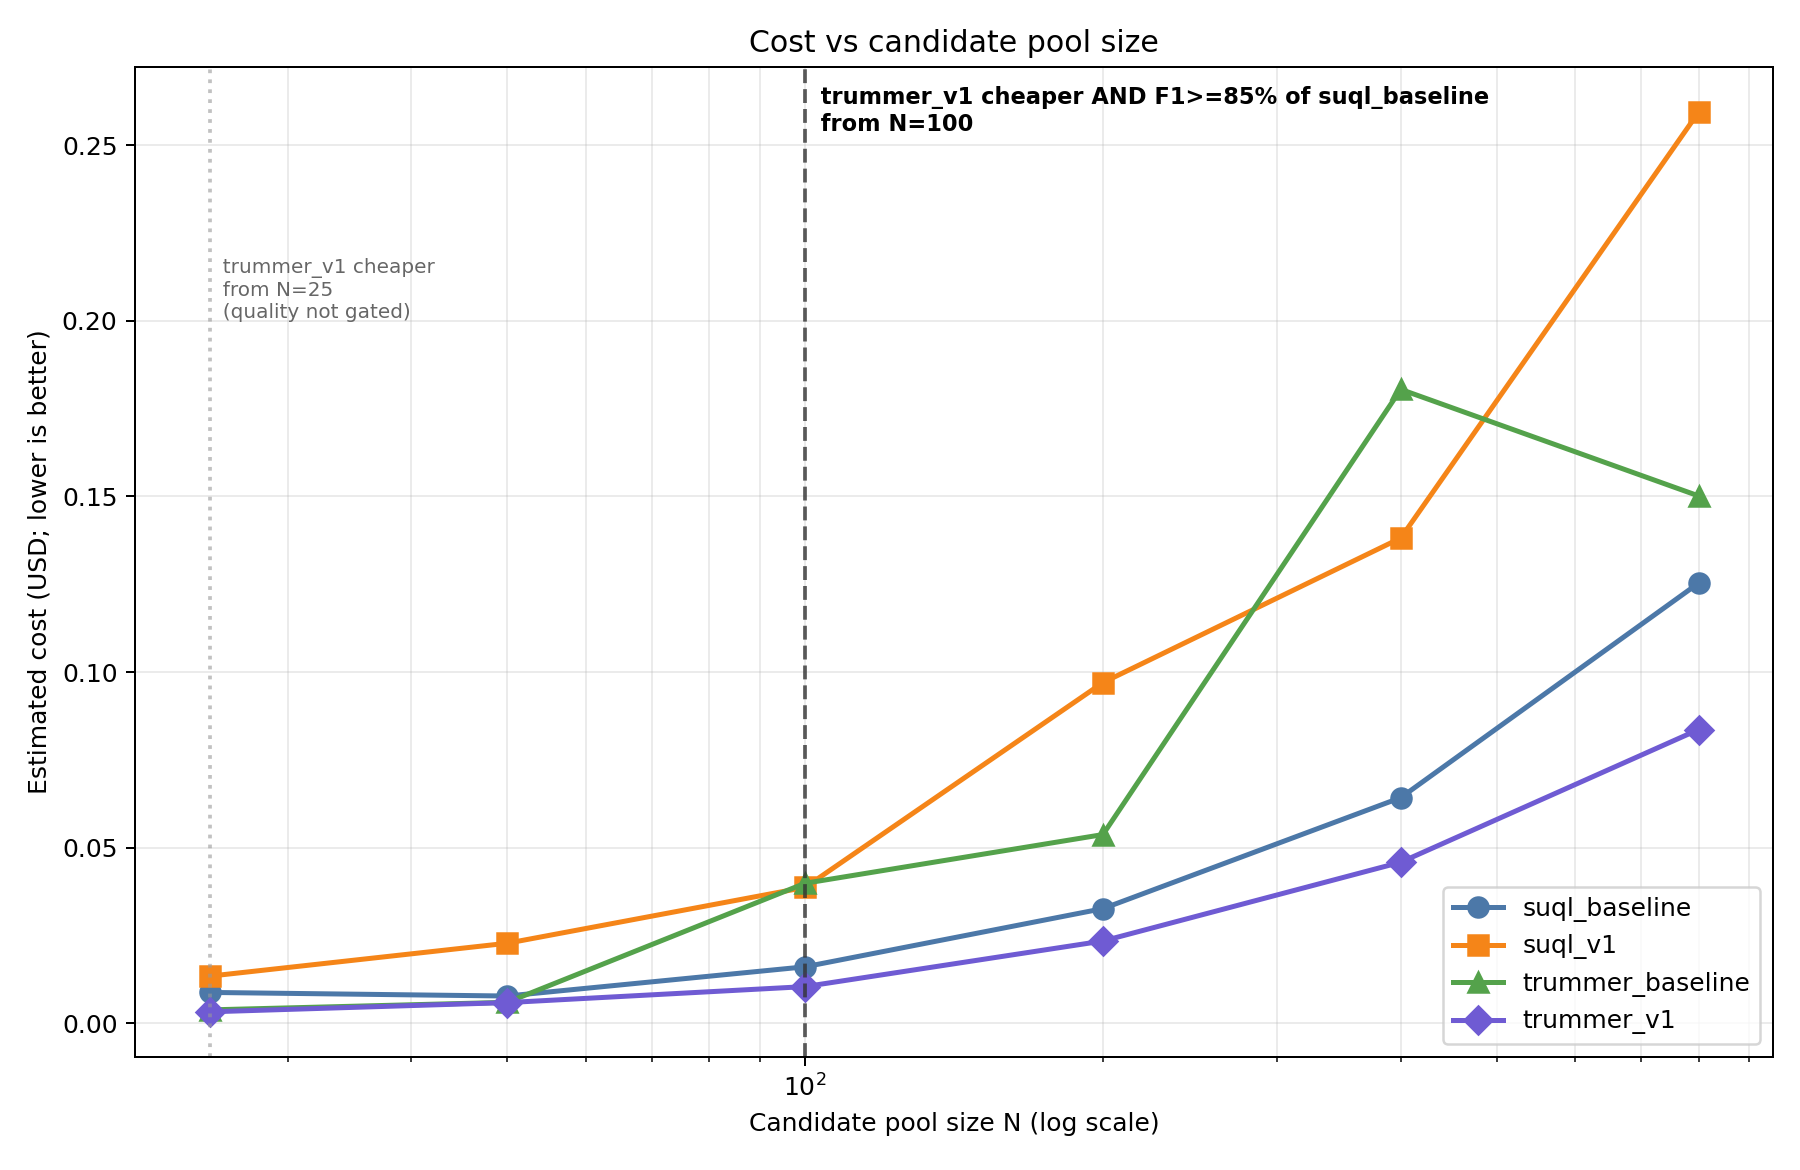
\includegraphics[width=0.85\textwidth]{figs/amazon/01_cost_vs_n.png}
\caption{Estimated \$-cost vs.\ candidate pool size $n$ (log scale),
all four methods.}
\label{fig:amzscale-cost}
\end{figure}

Figure~\ref{fig:amzscale-cost} sweeps pool size on a log axis; because
the underlying cost model is linear in $n$ plus a fixed calibration
term (Proposition~\ref{prop:crossover}), the near-flat-then-rising
shape here is the expected signature of a linear function viewed
against $\log n$, not evidence of super-linear growth. The annotated
threshold marks where Trummer~V1 becomes cheaper than SUQL baseline
(from $n{=}25$, quality not yet gated) and where it is both cheaper and
within $85\%$ of SUQL baseline's F1 ($n{=}100$).

\begin{figure}[h]
\centering
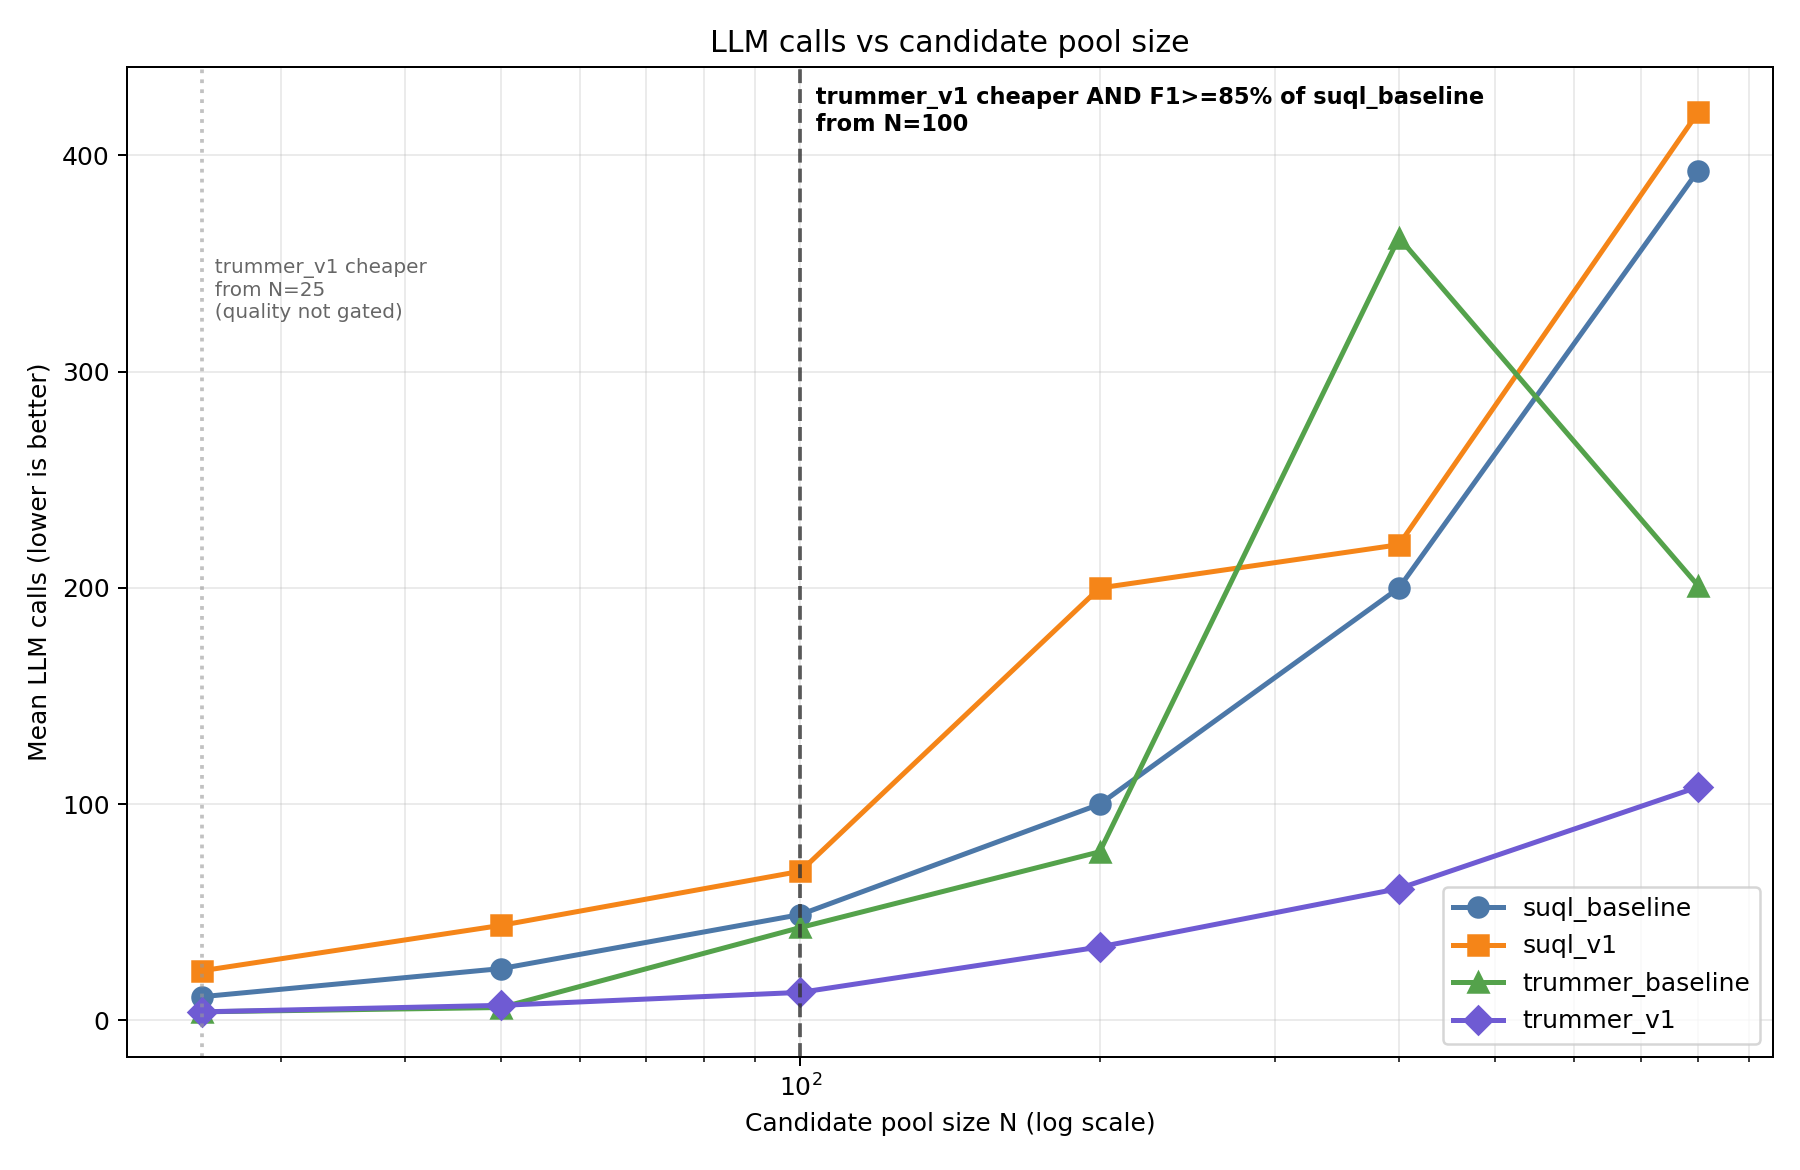
\includegraphics[width=0.85\textwidth]{figs/amazon/02_calls_vs_n.png}
\caption{Mean LLM calls vs.\ candidate pool size $n$ (log scale).}
\label{fig:amzscale-calls}
\end{figure}

Figure~\ref{fig:amzscale-calls} isolates raw call count from \$-cost.
Trummer~V1 (purple) is the lowest line at every $n$ tested; Trummer
baseline (green) is visibly the noisiest -- consistent with its
adaptive block-pairing retrying and re-partitioning depending on
parse success (Section~\ref{sec:trummer-baseline}), unlike the other
three methods' comparatively smooth, near-linear growth.

\begin{figure}[h]
\centering
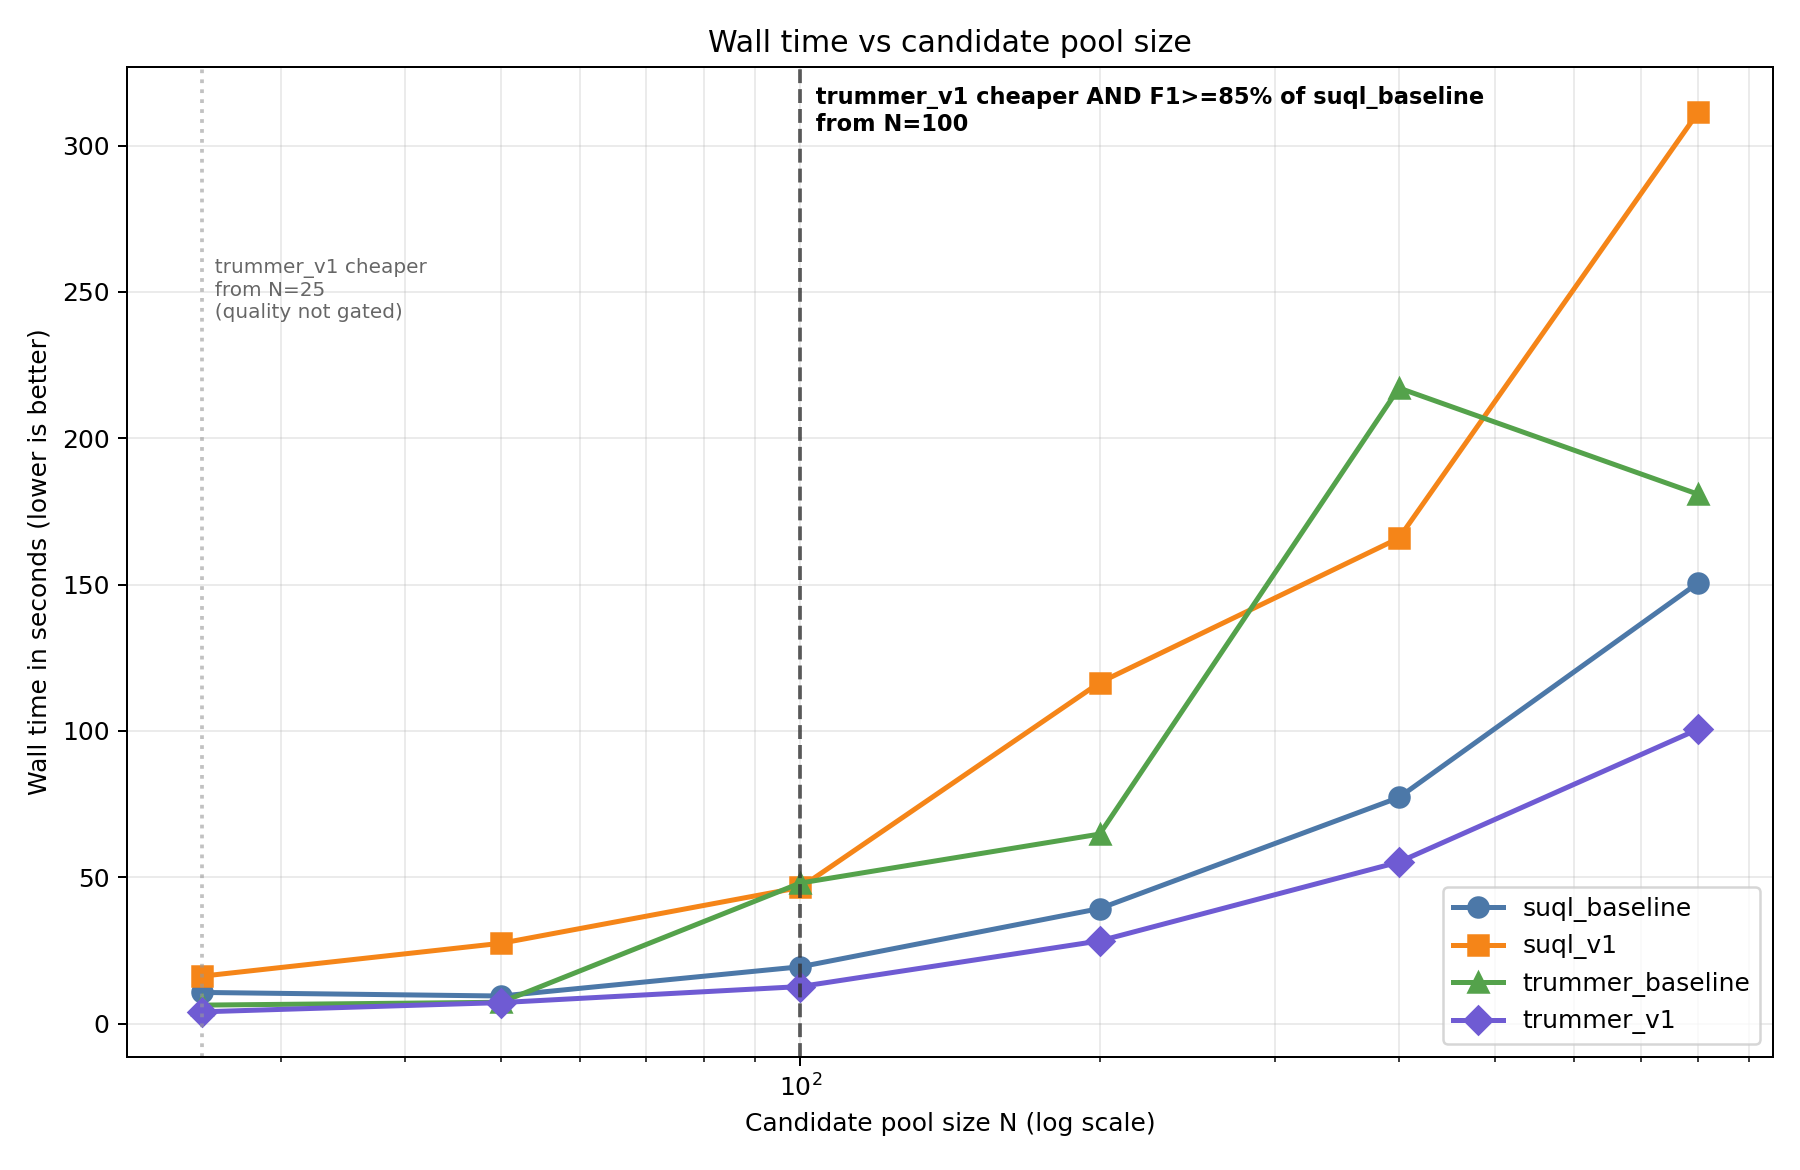
\includegraphics[width=0.85\textwidth]{figs/amazon/03_time_vs_n.png}
\caption{Mean wall time (s) vs.\ candidate pool size $n$ (log scale).}
\label{fig:amzscale-time}
\end{figure}

Figure~\ref{fig:amzscale-time} shows SUQL~V1 (orange) crossing above
even the noisy Trummer baseline by roughly $n{=}150$ and finishing as
the slowest method at $n{=}300$ -- the same qualitative story as the
IMDb result, now shown continuously across a wide range of pool sizes
rather than at one fixed $n$.

\begin{figure}[h]
\centering
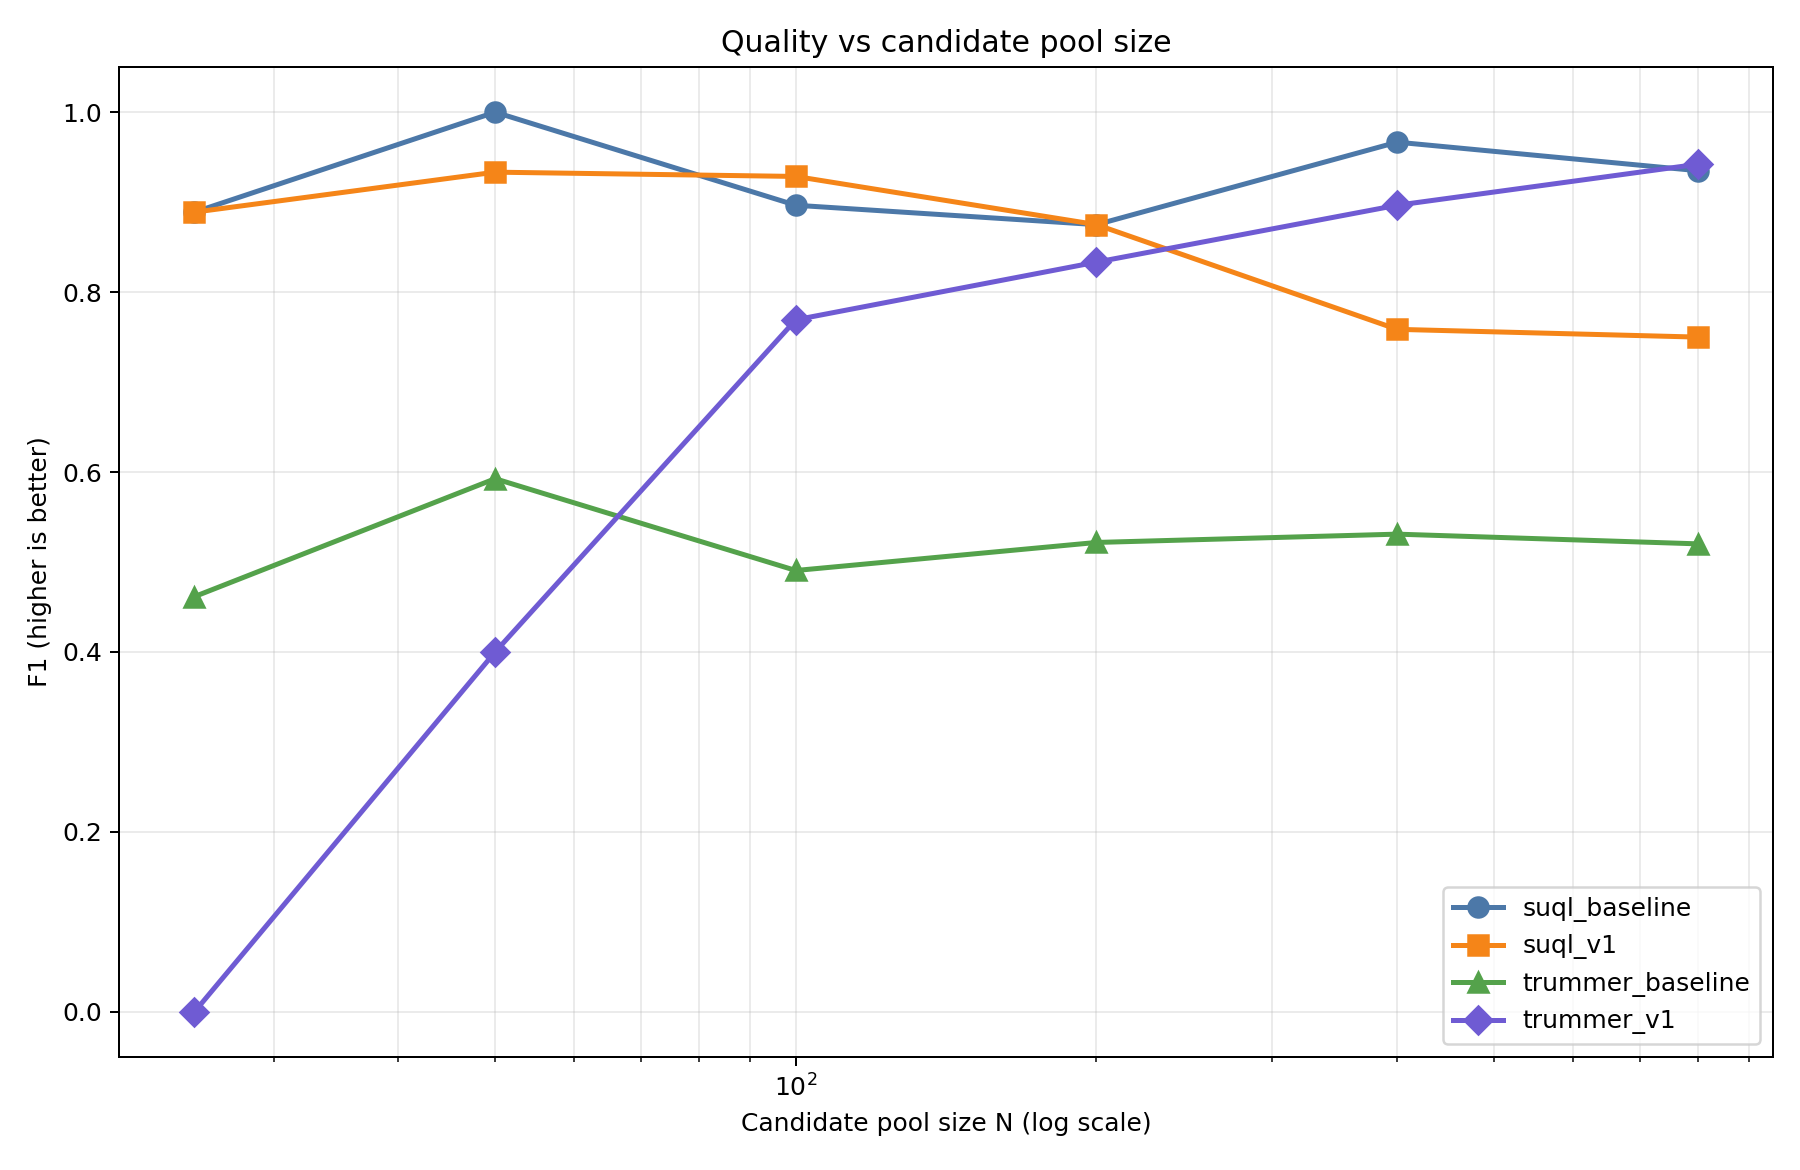
\includegraphics[width=0.85\textwidth]{figs/amazon/04_f1_vs_n.png}
\caption{F1 vs.\ candidate pool size $n$ (log scale).}
\label{fig:amzscale-f1}
\end{figure}

Figure~\ref{fig:amzscale-f1} is the least monotonic of the four: every
method's F1 line bends up and down across the sweep rather than
trending cleanly, and Trummer~V1 (purple) starts at F1 $=0$ for the
smallest pool tested before climbing above every other method by
$n{\gtrsim}150$. This non-monotonicity is discussed below -- it
reflects the escalation rate $\pi$ not being perfectly stable across
differently-sized synthetic pools, and, at the smallest $n$, the
calibration set itself being too small relative to $n$ for the
threshold search to produce a usable band at all.

Computing the empirical failure probability
$\Pr[\text{cascade cost}\ge\text{vanilla cost}]$ from every pairwise
comparison at each $n$: \textbf{on LLM calls, the cascade lost
\emph{zero} times, at every $n$ from $100$ to $300$, in both
regimes} -- including the adversarial one, meaning the measured margin
$\Delta$ beat even a calibration cost that never amortizes away. On
wall time, one small ($0.66\%$) failure rate appears at $n{=}100$,
vanishing by $n{=}125$, consistent with ordinary system-timing jitter.
One honest caveat: \texttt{expensive\_calls} had \emph{zero}
within-$n$ variance here (deterministic cheap-stage decoding), so this
confirms Proposition~\ref{prop:crossover}'s conclusion cleanly without
directly exercising Proposition~\ref{prop:hoeffding}'s Binomial-concentration
mechanism -- a follow-up with a sampling-temperature cheap stage or
freshly-resampled pools per repetition would be needed for that.

Quality is less clean across this sweep: Trummer~V1 loses F1 to the
lean vanilla reference at $2$ of $6$ pool sizes in the dense run and
$4$ of $6$ in calibfrac, tracking a \texttt{calibration\_agreement}
that misses its $0.9$ target at every single point tested ($0.27$--$0.89$).
This reinforces, independently of \S\ref{sec:imdb-vs-amazon-fashion}'s
ten-question comparison, that Trummer~V1's point-estimate calibration
(\S\ref{sec:trummer-v1}) is the more likely source of cross-domain
quality variability than the cascade architecture itself.

\subsection{Qwen vs.\ Gemma on Amazon}
\label{sec:amazon-model-comparison-2}

A Qwen cheap/expensive pair was evaluated on the same Amazon workload,
in a five-question-averaged suite. Table~\ref{tab:qwen-vs-gemma}
compares it against the Amazon Fashion \texttt{10q} Gemma run of
\S\ref{sec:imdb-vs-amazon-fashion} -- a better-matched reference than
the single pool-size point used in an earlier revision, though the
suite sizes still differ (five questions vs.\ ten).

\begin{figure}[h]
\centering

\includegraphics[width=0.85\textwidth]{figs/qwen_amazon/01_quality.png}
\caption{Qwen, Amazon five-question suite: precision, recall, F1
(error bars: std.\ dev.\ across repetitions).}
\label{fig:qwen-quality}
\end{figure}

Figure~\ref{fig:qwen-quality} shows the same precision/recall imbalance
for Trummer baseline under Qwen as under Gemma
(Figure~\ref{fig:amzf-quality}): precision collapses to $0.360$ against
recall $0.907$. SUQL baseline, SUQL~V1, and Trummer~V1 all cluster in a
narrow F1 band ($0.863$--$0.878$), with error bars overlapping
substantially -- the three are not clearly separable on quality alone
under this suite's repetition count.

\begin{figure}[h]
\centering

\includegraphics[width=0.85\textwidth]{figs/qwen_amazon/02_time.png}
\caption{Qwen, Amazon five-question suite: mean wall time, cheap vs.\
expensive stage.}
\label{fig:qwen-time}
\end{figure}

Figure~\ref{fig:qwen-time} again puts SUQL~V1 tallest ($48.3$s,
$77\%$ cheap-stage) and Trummer~V1 shortest ($17.4$s), the same
qualitative ranking as both Gemma runs above, now under a different
model family entirely.

\begin{figure}[h]
\centering

\includegraphics[width=0.85\textwidth]{figs/qwen_amazon/03_calls.png}
\caption{Qwen, Amazon five-question suite: mean LLM calls, cheap vs.\
expensive stage.}
\label{fig:qwen-calls}
\end{figure}

Figure~\ref{fig:qwen-calls} shows SUQL~V1 using \emph{more} total calls
than SUQL baseline ($75.0$ vs.\ $48.6$), matching its Amazon-Fashion
behavior under Gemma (Figure~\ref{fig:amzf-calls}) rather than its
IMDb behavior -- further evidence that the IMDb result was closer to a
best case for SUQL~V1 than a typical one.

\begin{figure}[h]
\centering

\includegraphics[width=0.85\textwidth]{figs/qwen_amazon/04_best_solution.png}
\caption{Qwen, Amazon five-question suite: recall vs.\ wall time,
harness best-solution annotation is Trummer~V1.}
\label{fig:qwen-best}
\end{figure}

Figure~\ref{fig:qwen-best} places all three of SUQL baseline, Trummer
baseline, and Trummer~V1 at broadly similar recall, with SUQL~V1 alone
pulled far to the right on time -- the same isolated-outlier pattern
seen in both Gemma figures (Figures~\ref{fig:imdb-best},
\ref{fig:amzf-best}).

\begin{figure}[h]
\centering

\includegraphics[width=0.85\textwidth]{figs/qwen_amazon/05_cost_by_approach.png}
\caption{Qwen, Amazon five-question suite: estimated \$-cost per
question.}
\label{fig:qwen-cost}
\end{figure}

Figure~\ref{fig:qwen-cost} shows SUQL~V1 as the most expensive method
(\$0.0403) and Trummer~V1 the cheapest (\$0.0145). The per-call
annotations are the basis of the cross-model \$-cost puzzle resolved
below: SUQL~V1's cheap-call cost here (\$0.00062) is identical to its
Gemma/Amazon-Fashion counterpart to five significant figures.

\begin{figure}[h]
\centering

\includegraphics[width=0.85\textwidth]{figs/qwen_amazon/06_cost_vs_f1.png}
\caption{Qwen, Amazon five-question suite: cost--F1 Pareto frontier.}
\label{fig:qwen-pareto}
\end{figure}

Figure~\ref{fig:qwen-pareto} shows the same two-point Pareto frontier
shape as the Gemma/Amazon-Fashion result (Figure~\ref{fig:amzf-pareto}):
Trummer~V1 (\$0.0145, F1 $0.865$) and SUQL baseline (\$0.0175, F1
$0.878$) are both non-dominated, while SUQL~V1 and Trummer baseline are
each dominated on both axes at once.

\begin{table}[h]
\centering\small
\begin{tabular}{lrr}
\toprule
vs.\ SUQL baseline & Qwen (5q) & Gemma (Amazon Fashion, 10q) \\
\midrule
Trummer~V1 $\Delta$F1    & $-1.5\%$  & $-4.3\%$ \\
Trummer~V1 $\Delta$calls & $-80.7\%$ & $-73.6\%$ \\
SUQL~V1 $\Delta$F1       & $-1.7\%$  & $-7.1\%$ \\
SUQL~V1 $\Delta$calls    & $+54.3\%$ & $+59.1\%$ \\
\bottomrule
\end{tabular}
\caption{Both model families now cover all four methods on Amazon data.}
\label{tab:qwen-vs-gemma}
\end{table}

The two model families now agree on \emph{direction} for every
comparison in the table, which they did not in an earlier revision of
this report (that revision's Gemma reference point showed a small
\emph{positive} F1 delta for Trummer~V1, based on one pool-size
measurement rather than a ten-question average; the properly-matched
comparison here shows a small \emph{negative} delta, consistent with
Qwen -- we flag this as a correction rather than silently updating it).
\textbf{Both model families show Trummer~V1 trading a small, consistent
amount of F1 ($1.5$--$4.3\%$) for a large, consistent reduction in
calls ($74$--$81\%$), and both show SUQL~V1 strictly dominated by its
own baseline on Amazon data} -- worse on calls, time, and F1 at once.
This is the clearest cross-model evidence in either report that the
cost mechanism (structured pushdown, batching) is architecture-level
and portable, while SUQL~V1's specific unbatched design is the outlier
that does not travel well.

A puzzle from an earlier revision of this report is now resolved rather
than merely flagged: SUQL~V1's reported per-call \$-cost is nearly
identical across the Qwen and Gemma Amazon runs (cheap $\$0.00062$ in
both; expensive $\$0.00036$ vs.\ $\$0.00033$). Section~\ref{sec:imdb-plots}'s
IMDb \$-cost breakdown confirms the mechanism: this harness's \$-cost
estimate is simply recorded model service \emph{time} multiplied by a
flat \$3.00/accelerator-hour rate, with no per-model price
differentiation, so two runs with similar per-call \emph{latency} will
show similar \$-costs regardless of which underlying model produced
that latency. The near-identical figures are therefore evidence that
SUQL~V1's cheap-stage latency happened to be similar under both model
labels, not evidence that the two runs shared an underlying model.

\paragraph{Remaining scope.} Neither run reports specific model
parameter counts (only ``cheap''/``expensive'' role labels), so the
exact ratio $P_c/P_e$ cannot yet be stated for the Qwen pair the way
Table~\ref{tab:theory-constants} does for Gemma. Both model families
now cover all four methods on Amazon data, closing the coverage gap
noted in an earlier revision of this report.

\section{Discussion}

\textbf{Structured selectivity still dominates wall time.} Across all
four variants, and now confirmed over ten diverse questions rather than
one, the wall-clock gap between the SUQL and Trummer families tracks how
many rows survive structured pushdown before any semantic operator runs;
every question in this suite fixes the structured candidate count at
$40$ out of $100$, so the ranking we report is specific to this
$40\%$-selectivity regime and should be re-measured at other
selectivities before being treated as universal.

\textbf{The \answerfn{} yield rate remains a useful label-free
diagnostic}, unchanged from earlier analysis: very high acceptance
of structurally-filtered rows indicates an under-specified predicate,
very low acceptance suggests over-constraint or a vocabulary mismatch,
and both are visible without any gold labels at all.

\textbf{\texttt{LIMIT} without early termination} remains an
unaddressed, self-contained optimization opportunity: none of the four
implementations currently stop evaluating the semantic operator early
once a \texttt{LIMIT k} clause's target has been met.

\textbf{Threats to validity, updated.} The \texttt{10q} suite directly
answers the single-query threat flagged previously, but a new,
narrower one appears in its place: every question in this suite shares
the same $100/40/12$ structural shape by design, so the reported
numbers characterize behavior at one fixed selectivity and one fixed
gold-set size, not a selectivity sweep. The repository's \texttt{1q},
\texttt{3q}, and \texttt{5q} suites, and the previously sketched
20-query ablation, remain the natural next steps toward a full
selectivity-by-difficulty grid (Chapter~\ref{chap:conclusion}).
